\section{Resultados}

\subsection{Teste de latência}

Para avaliar a latência da comunicação em tempo real entre o aplicativo \textit{mobile} e o \textit{backend}, foi realizada uma coleta durante sessões de corrida online. A instrumentação adicionada ao sistema registrou, para cada mensagem biométrica enviada pelo aplicativo, um identificador único de rastreamento (\texttt{latencyTraceId}), o instante de envio no cliente, o tempo de processamento no \textit{backend} e o tempo total observado até o retorno do estado do jogo ao \textit{mobile}. Dessa forma, cada amostra de latência foi correlacionada diretamente entre o \textit{log} do aplicativo Android e o \textit{log} do \textit{backend}, evitando inferências baseadas apenas na ordem das mensagens.

O teste de latência foi realizado para verificar se a comunicação entre o aplicativo móvel e o \textit{backend} seria rápida o suficiente para sustentar a experiência de corrida gamificada em tempo real. Como o funcionamento do sistema depende do envio contínuo de informações do usuário, como distância percorrida, velocidade e dados biométricos, era necessário garantir que o estado da corrida retornasse ao aplicativo sem atrasos perceptíveis. Durante uma sessão de uso, o aplicativo envia dados ao servidor, o \textit{backend} processa essas informações, atualiza a posição do usuário e da horda e devolve ao aplicativo o novo estado do jogo. Esse ciclo precisa acontecer de maneira frequente, pois qualquer atraso excessivo poderia comprometer a sensação de continuidade da corrida e prejudicar a percepção do usuário sobre a aproximação da horda.

Na coleta analisada, foram registrados 25 rastreamentos de latência no \textit{backend} e os mesmos 25 rastreamentos no aplicativo \textit{mobile}, sem perda de mensagens entre os dois lados. A Tabela~\ref{tab:latencia-geral} apresenta os resultados gerais da latência ponta a ponta, considerando o caminho do \textit{mobile} ao \textit{backend} e o retorno ao \textit{mobile}, bem como o tempo de processamento interno do \textit{backend}.

\begin{table}[!ht]
    \centering
    \caption{Resultados gerais da medição de latência}
    \label{tab:latencia-geral}
    \begin{adjustbox}{max width=\columnwidth}
    \begin{tabular}{lccccc}
        \hline
        \textbf{Métrica} & \textbf{Amostras} & \textbf{Mín.} & \textbf{Média} & \textbf{Mediana} & \textbf{Máx.} \\
        \hline
        Ponta a ponta & 25 & 20 ms & 27,64 ms & 22 ms & 110 ms \\
        Backend & 25 & 10 ms & 14,44 ms & 14 ms & 24 ms \\
        \hline
    \end{tabular}
    \end{adjustbox}
\end{table}

Também foi calculado o percentil 95 das amostras. Para a latência ponta a ponta, o p95 foi de 47 ms, enquanto que, para o processamento interno do \textit{backend}, o p95 foi de 19 ms. O maior valor observado na latência ponta a ponta foi de 110 ms, ocorrido na primeira mensagem da primeira sessão. Como esse ponto ficou acima do comportamento observado nas demais mensagens, ele foi interpretado como um possível efeito de aquecimento da conexão e de inicialização do fluxo de comunicação.

Ao remover apenas essa primeira amostra, a latência em regime mais estável apresentou uma média de 24,21 ms, mediana de 22 ms, p95 de 32 ms e valor máximo de 47 ms em 24 amostras. Esse resultado indica que, após a estabilização inicial, a comunicação em tempo real manteve tempos baixos e consistentes para a atualização do estado do jogo no aplicativo.

\begin{table}[!ht]
    \centering
    \caption{Latência ponta a ponta por sessão}
    \label{tab:latencia-sessao}
    \begin{adjustbox}{max width=\columnwidth}
    \begin{tabular}{lcccc}
        \hline
        \textbf{Sessão} & \textbf{Amostras} & \textbf{Média} & \textbf{Mediana} & \textbf{Máx.} \\
        \hline
        \texttt{9fd8f4c7...} & 6 & 37,33 ms & 22,5 ms & 110 ms \\
        \texttt{8d63db71...} & 6 & 24,17 ms & 23,5 ms & 30 ms \\
        \texttt{cd9d094c...} & 6 & 25,00 ms & 20,5 ms & 47 ms \\
        \texttt{1c03cac3...} & 6 & 24,57 ms & 24 ms & 32 ms \\
        \hline
    \end{tabular}
    \end{adjustbox}
\end{table}
A quantidade de 6 amostras por sessão na Tabela~\ref{tab:latencia-sessao} representa as requisições de telemetria que foram enviadas nos primeiros 5 segundos de cada sessão de teste, sendo uma requisição por segundo aproximadamente. Esses ensaios preliminares foram conduzidos no início do desenvolvimento para avaliar a viabilidade prática do projeto, analisando a latência ponta a ponta no envio e processamento dos dados. O fluxo percorrido inicia com a frequência cardíaca coletada pelo \textit{smartwatch}, enviada ao celular via \textit{Bluetooth}, transmitida ao \textit{backend} por rede sem fio, processada no servidor e devolvida para exibição no dispositivo final.

Os resultados obtidos apresentaram tempos de latência muito menores do que o esperado. Inicialmente, as medições foram executadas utilizando rede \textit{Wi-Fi} local e com os dispositivos estáticos. Para validar a comunicação em condições reais de mobilidade, foram realizados testes adicionais utilizando rede móvel 5G. A transição para a rede móvel não causou impacto significativo nos tempos medidos, mantendo as médias de resposta estáveis e próximas às obtidas em rede local. Isso confirma que a arquitetura e os protocolos adotados são plenamente viáveis para garantir a comunicação em tempo real desejada.

Os resultados indicam que o \textit{backend} teve baixo impacto no tempo total de resposta, com processamento médio de 14,44 ms. Convém destacar que o servidor foi hospedado remotamente utilizando um \textit{Droplet} da \textit{DigitalOcean}. Mesmo com a comunicação trafegando pela internet pública até a nuvem e retornando ao dispositivo, a maior parte da latência ponta a ponta (média de 27,64 ms) esteve associada ao ciclo completo de envio da telemetria, processamento no servidor, publicação do novo estado via \textit{WebSocket}/\textit{STOMP} e recebimento pelo aplicativo. Mesmo considerando o maior valor observado, a latência permaneceu inferior a 120 ms, o que é adequado para a interação proposta, dado que o aplicativo atualiza o estado da corrida em ciclos de aproximadamente um segundo. Desse modo, as medições de tempo confirmam que o sistema atende aos requisitos de sincronização entre o usuário, a horda e a interface do aplicativo móvel, demonstrando o bom desempenho da infraestrutura em nuvem adotada.

\subsection{Teste de usabilidade}

A avaliação de usabilidade teve como objetivo verificar se os principais fluxos da aplicação são compreensíveis para o usuário e se a proposta de gamificação é percebida de forma clara durante a interação. Foram considerados os fluxos de autenticação, seleção de horda, início da corrida, acompanhamento da sessão, visualização do estado do \textit{smartwatch} e encerramento da atividade. Durante a análise, observou-se que a divisão da aplicação em telas específicas contribui para a compreensão do fluxo geral. A Figura~\ref{fig:fluxo_telas} ilustra o fluxo de navegação e as etapas principais do aplicativo móvel, abrangendo o acesso, a área principal, a pré-corrida, a corrida e as telas auxiliares. A tela inicial concentra a seleção da horda, a distância-alvo, o estado de conexão do relógio e o início da sessão. A tela do jogo apresenta o progresso da corrida, o estado remoto da sessão, a pressão exercida pela horda e os dados de telemetria. Já o relógio atua como uma extensão da experiência, exibindo informações resumidas, como batimentos por minuto, progresso, risco e estado de sincronização com o celular.

\begin{figure*}[t]
    \centering
    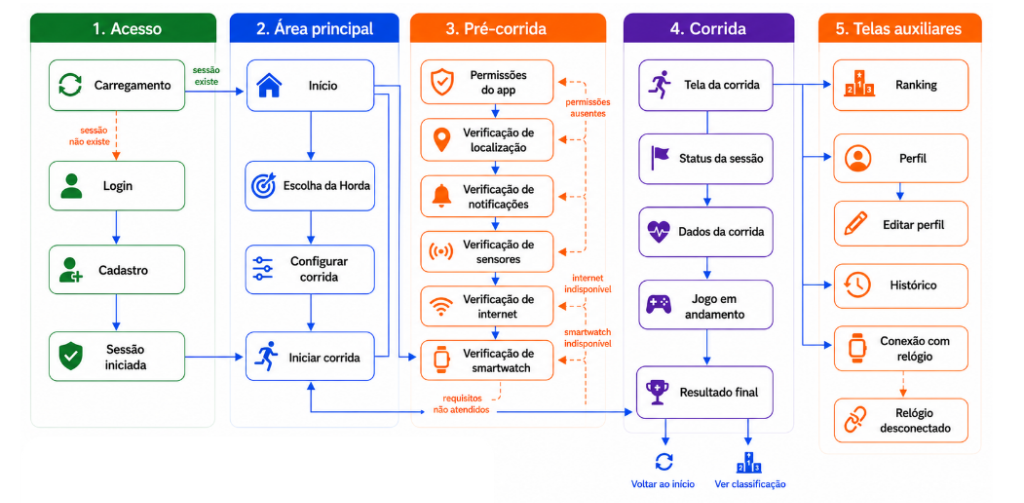
\includegraphics[width=0.9\textwidth]{figuras/fluxo_telas.png}
    \captionsetup{justification=centering}
    \caption{Fluxo de telas e navegação do aplicativo móvel.}
    \label{fig:fluxo_telas}
\end{figure*}

A presença de indicadores visuais de estado, como sessão ativa, relógio conectado ou desconectado e progresso da corrida, auxilia o usuário a compreender se o sistema está pronto para iniciar a atividade. Além disso, a sincronização automática entre celular e relógio reduz a necessidade de ações manuais no \textit{smartwatch}, tornando o fluxo mais simples durante o início e o encerramento da horda.

Durante a fase de verificação técnica, também foram observadas limitações relacionadas ao uso do \textit{smartwatch} como dispositivo complementar. Por se tratar de uma aplicação \textit{Wear OS}, houve a necessidade de considerar restrições próprias do \textit{hardware} do relógio, como menor capacidade de processamento, tela reduzida e maior cuidado com o consumo de recursos. Essas limitações influenciaram diretamente a forma de exibição das informações no relógio, priorizando dados resumidos e essenciais, como batimentos por minuto, progresso e estado de conexão, em vez de interfaces mais complexas.

Outro desafio identificado foi a visualização e conferência dos dados de telemetria durante as corridas. Como parte das informações era coletada em tempo real e transmitida entre relógio, celular e \textit{backend}, a validação exigiu o acompanhamento simultâneo dos estados exibidos na interface, dos registros de comunicação e das respostas recebidas do servidor. Esse processo evidenciou a importância de manter indicadores claros na interface e registros consistentes para auxiliar na verificação do comportamento do sistema durante a validação técnica.

Como limitação, a avaliação ainda não contempla uma amostra ampla de usuários externos nem a aplicação formal de questionários padronizados, como o User Experience Questionnaire (UEQ). Assim, os resultados de usabilidade apresentados nesta etapa têm caráter exploratório e se concentram na validação dos fluxos principais implementados, bem como na identificação de dificuldades práticas de interação entre usuário, aplicativo móvel e \textit{smartwatch}.

\subsection{Análise funcional}

A análise funcional foi realizada a partir dos fluxos implementados no aplicativo móvel, no \textit{smartwatch} e no \textit{backend}. O objetivo foi verificar se os componentes do sistema operam de forma integrada e se os contratos de comunicação entre as partes permanecem consistentes durante uma sessão de corrida online. No \textit{backend}, foram validados os fluxos de autenticação, criação de sessão, carregamento de hordas, recebimento de dados biométricos, atualização do \textit{ranking}, cálculo da posição virtual da horda e publicação do estado do jogo via \textit{WebSocket}. O servidor atua como fonte de verdade da sessão online, determinando os estados \texttt{RUNNING}, \texttt{CAUGHT} e \texttt{ESCAPED}.

No aplicativo móvel, foram verificados os fluxos de \textit{login}, seleção de horda, início da corrida, coleta de telemetria, envio periódico de dados ao \textit{backend}, recepção do estado remoto e renderização visual da corrida. A cena do jogo não calcula de forma independente o resultado da sessão, ela representa visualmente o estado recebido do \textit{backend}, reduzindo inconsistências entre a lógica da corrida e a interface apresentada ao usuário.

\begin{figure*}[!t]
    \centering
    \begin{minipage}{0.48\textwidth}
        \centering
        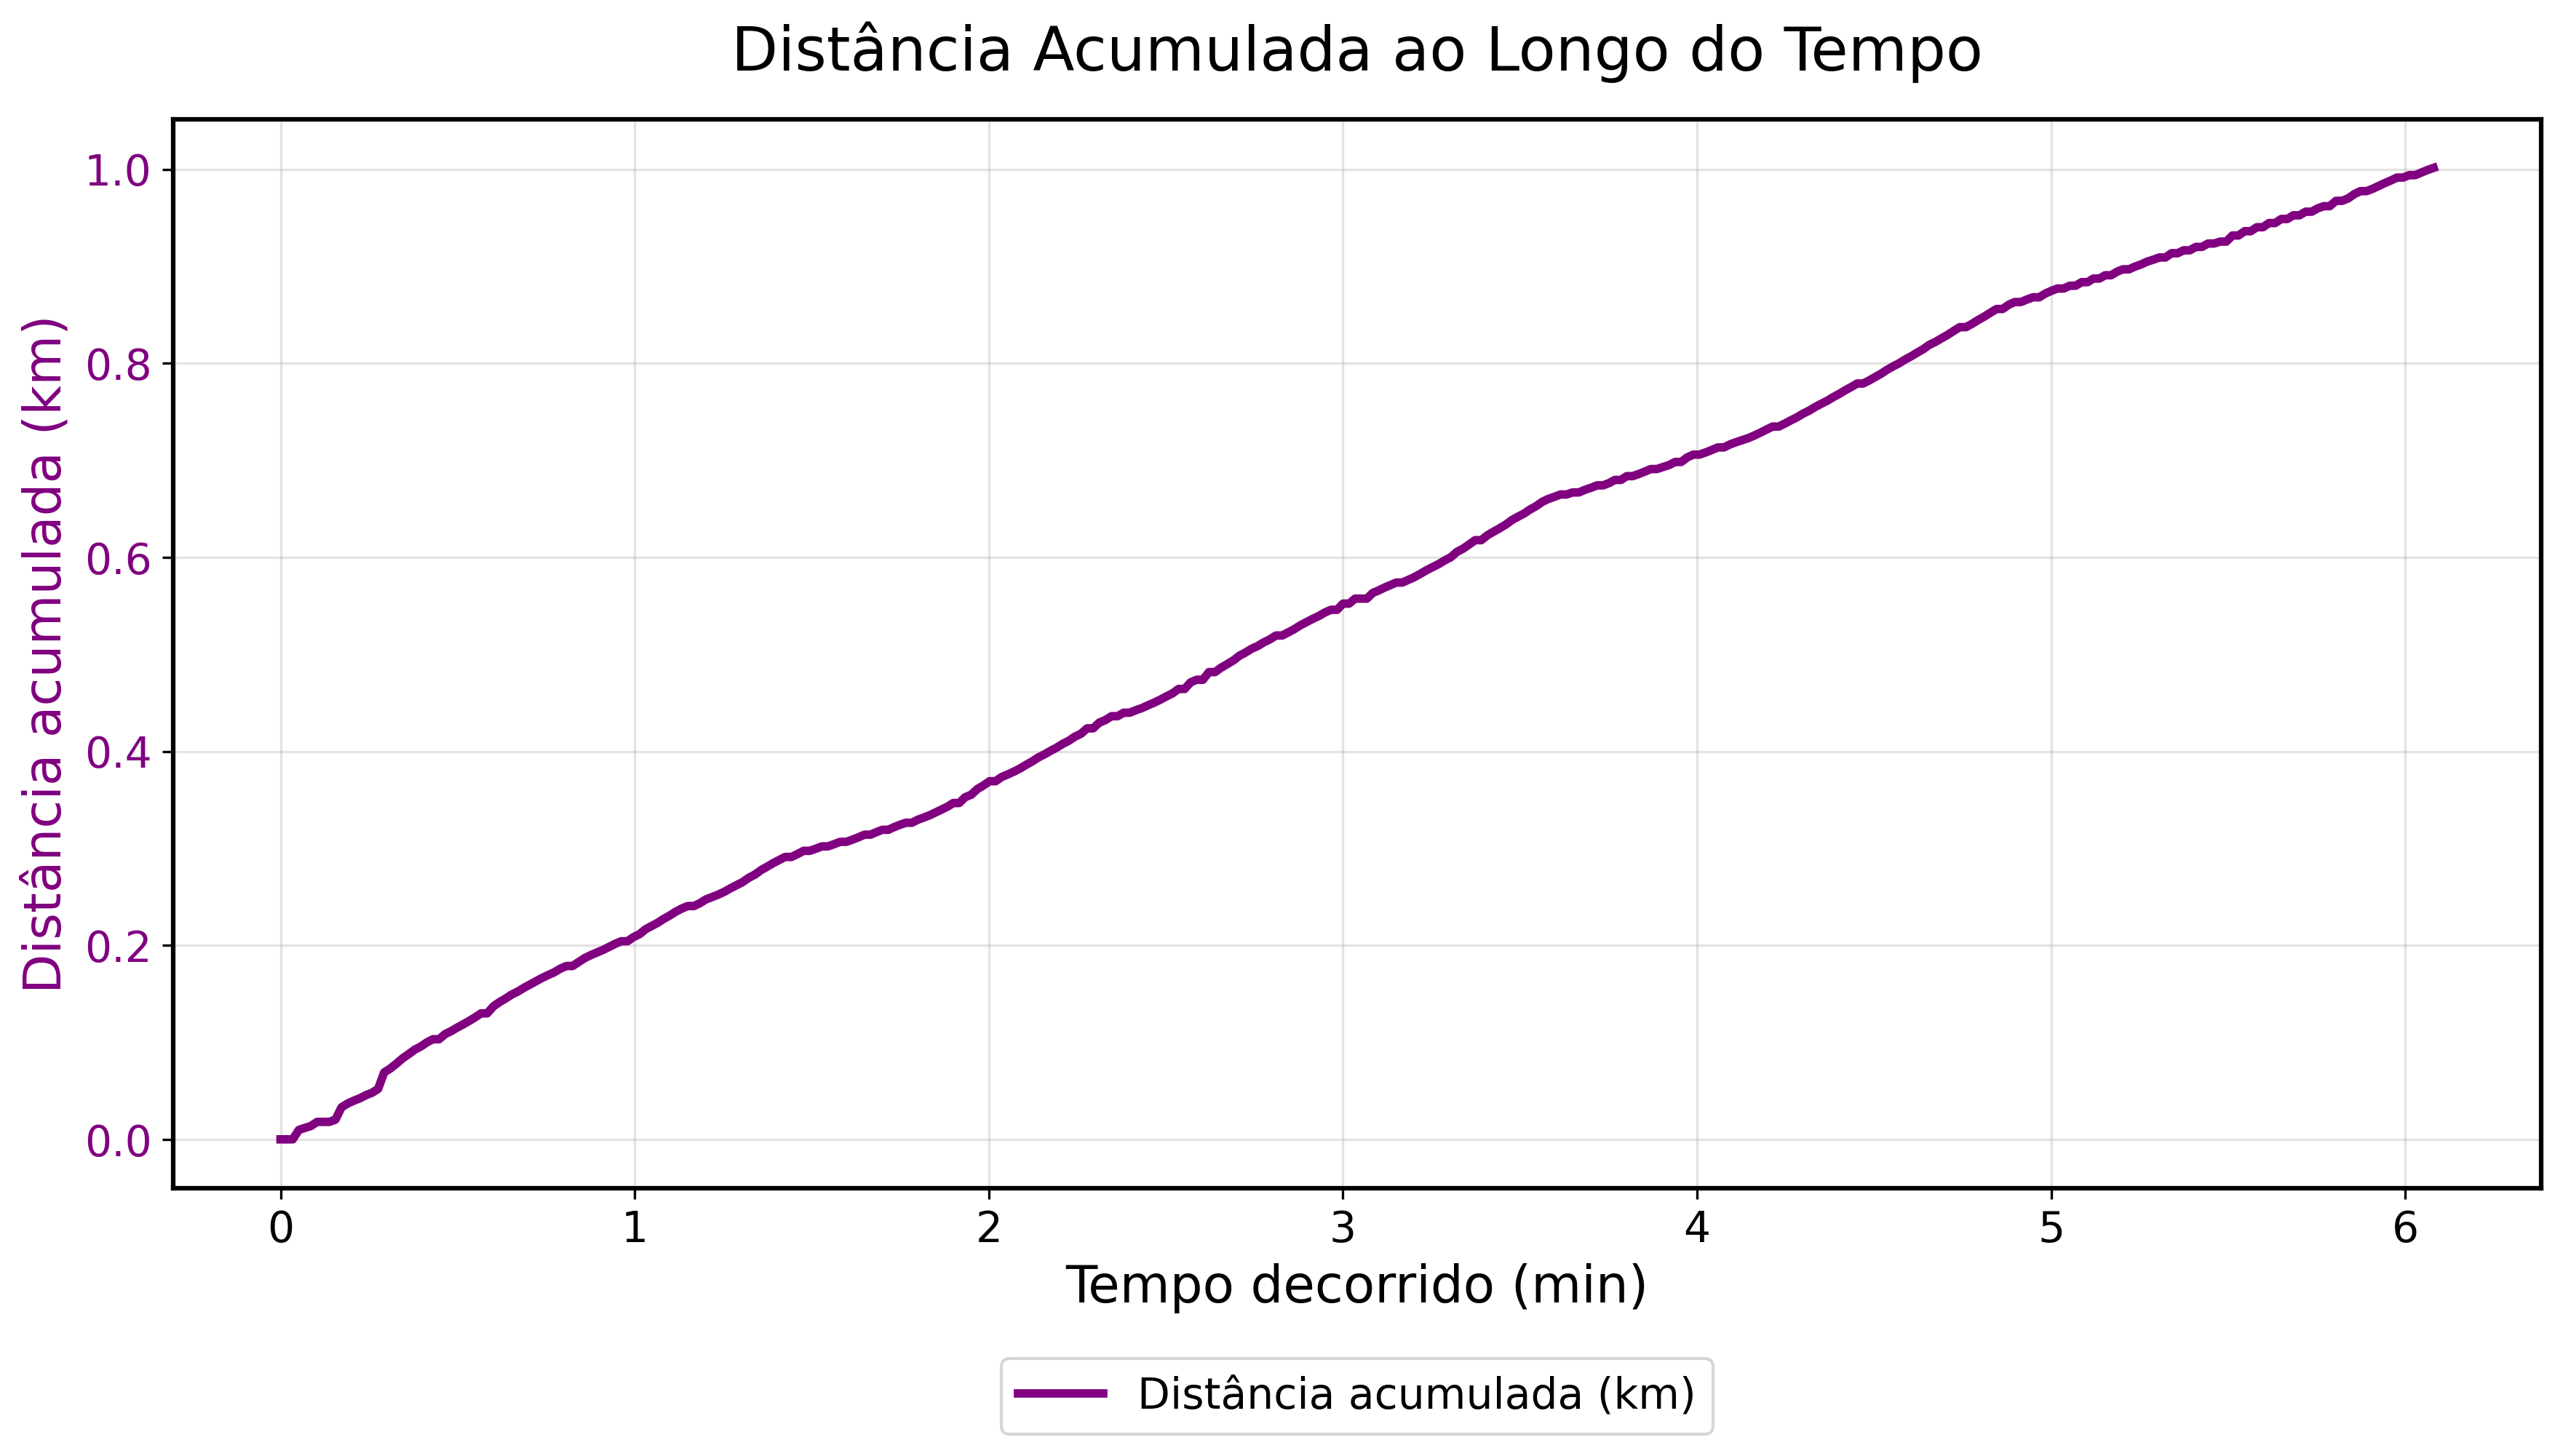
\includegraphics[width=\textwidth]{figuras/grafico_distancia_visivel.png}
        \captionsetup{justification=centering}
        \caption{Distância acumulada registrada durante a execução da corrida.}
        \label{fig:grafico_distancia}
    \end{minipage}
    \hfill
    \begin{minipage}{0.48\textwidth}
        \centering
        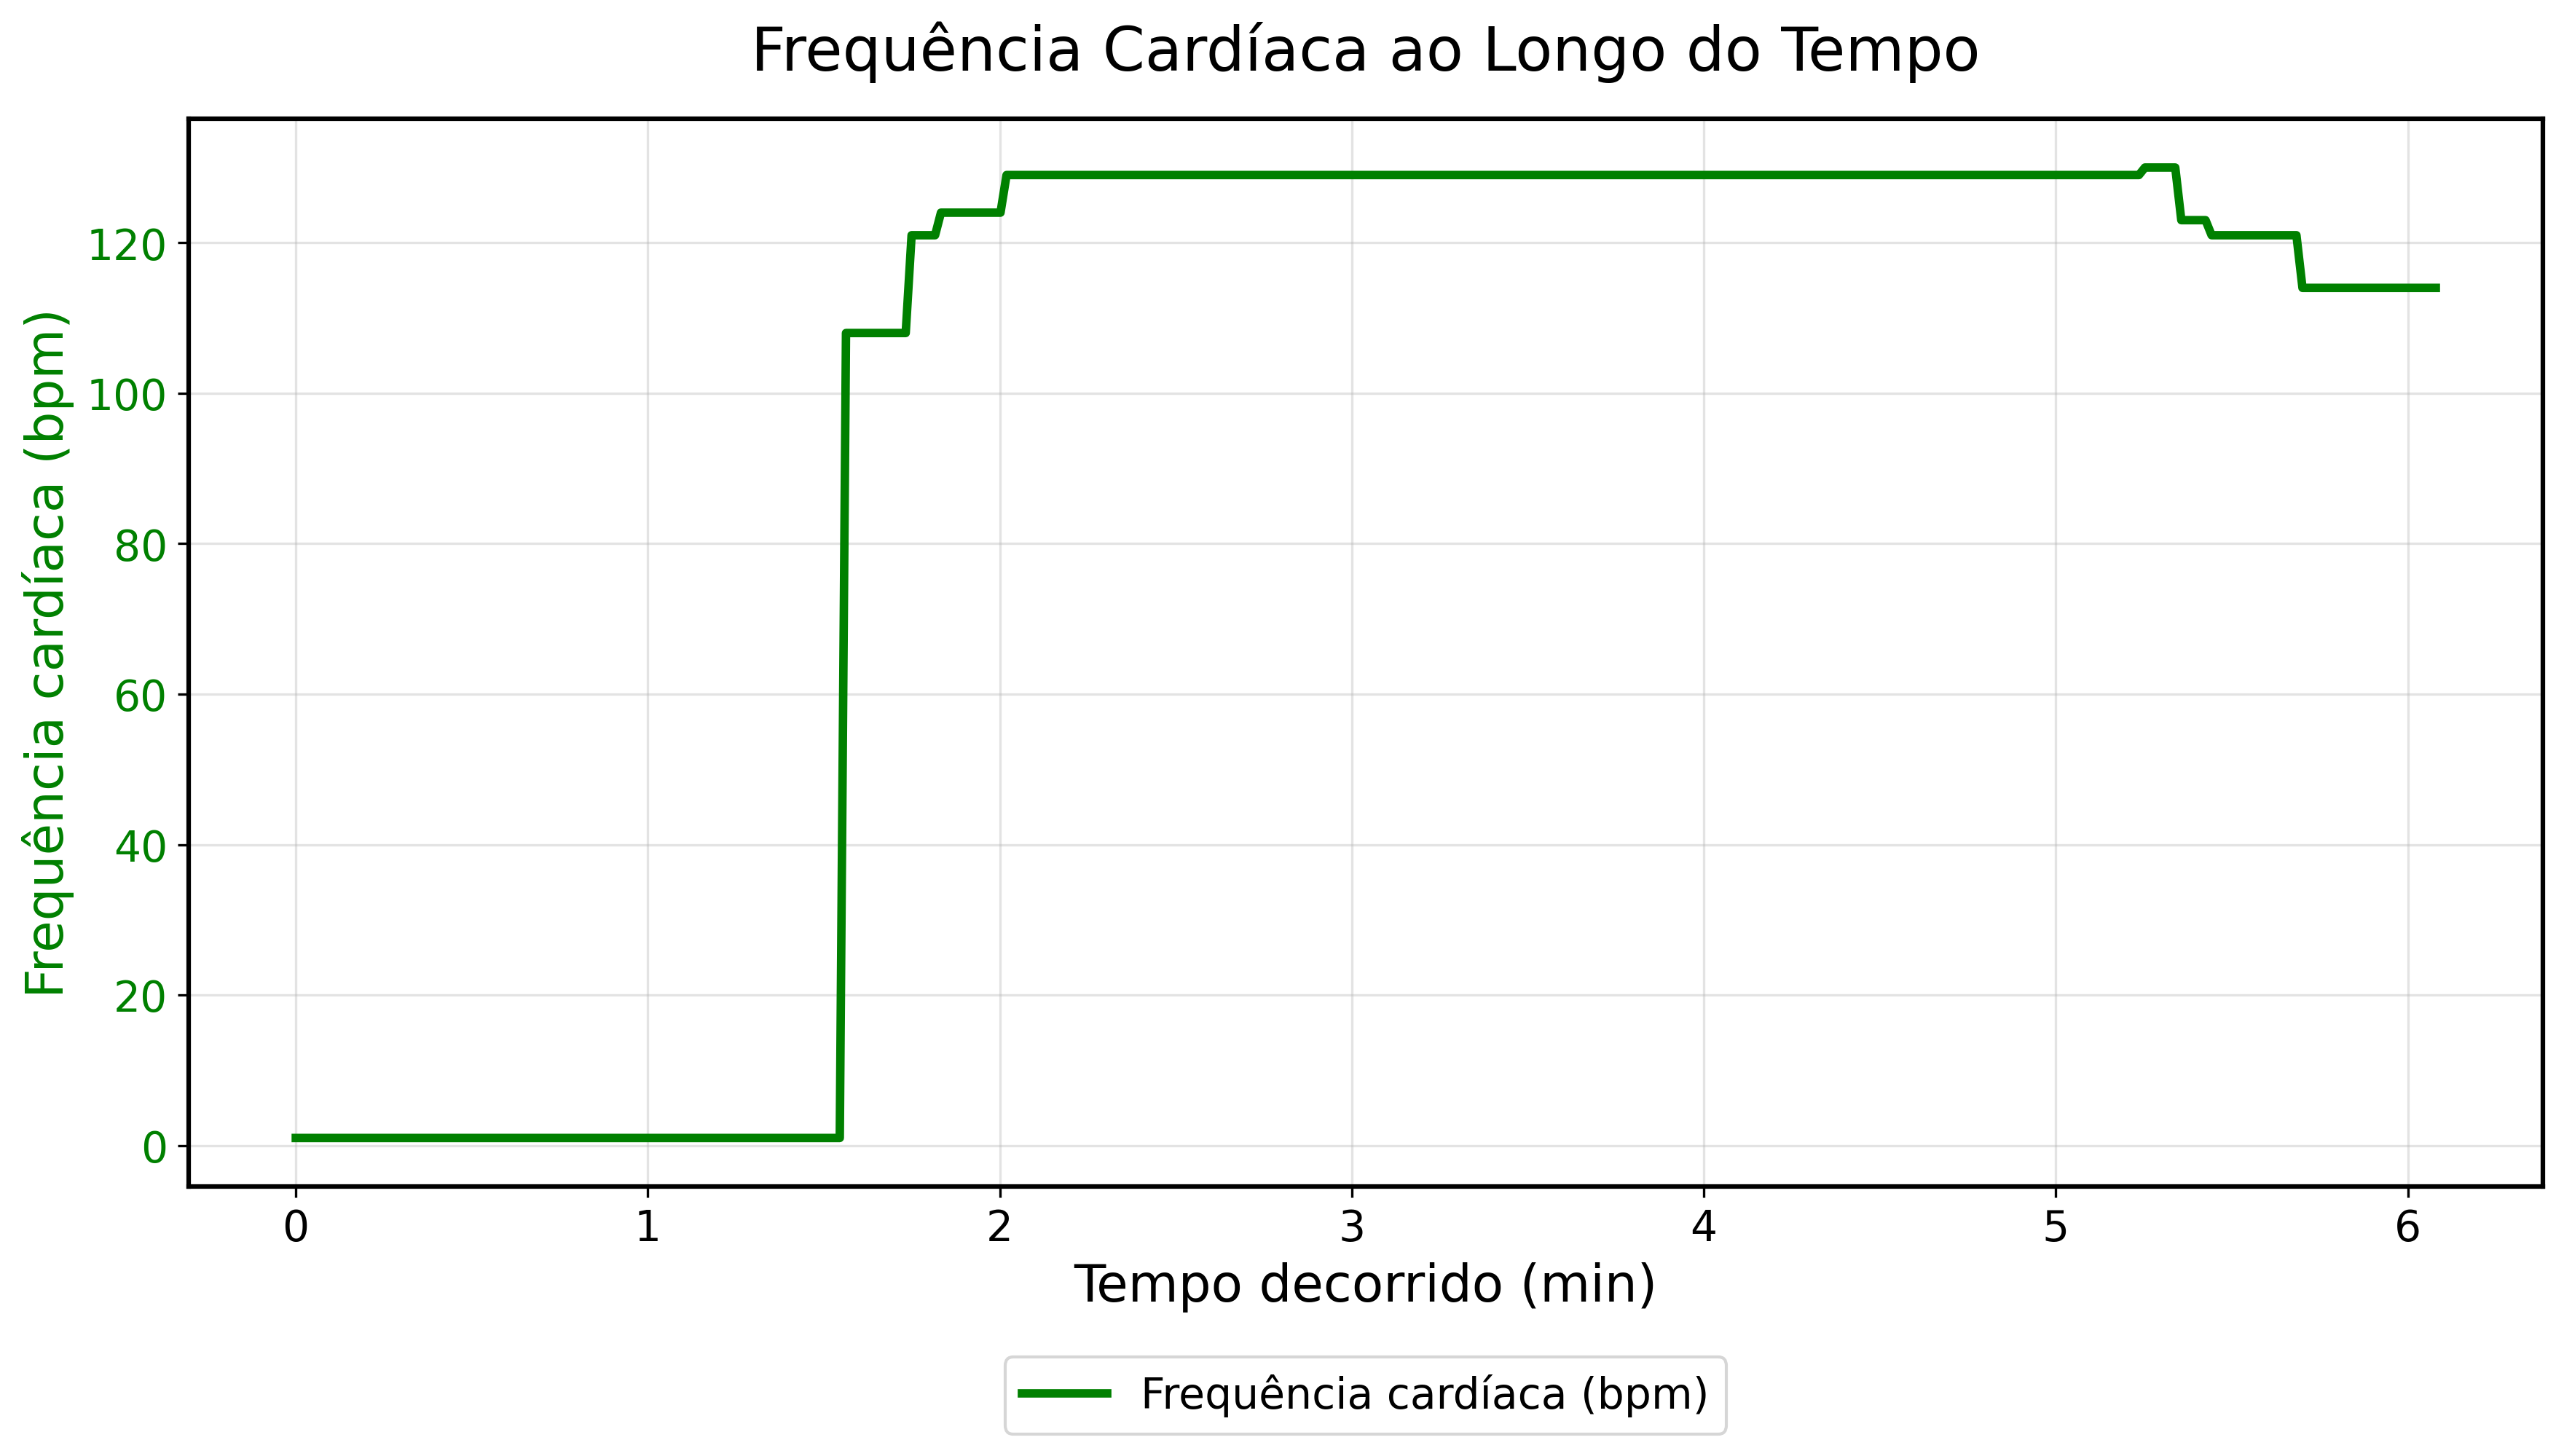
\includegraphics[width=\textwidth]{figuras/grafico_frequencia_cardiaca_visivel.png}
        \captionsetup{justification=centering}
        \caption{Frequência cardíaca coletada pelo \textit{smartwatch} durante a sessão de corrida.}
        \label{fig:grafico_frequencia}
    \end{minipage}
\end{figure*}

A Figura~\ref{fig:grafico_distancia} apresenta a distância acumulada registrada durante a execução da corrida. Esse dado é essencial para acompanhar o avanço do usuário durante a sessão e também serve como base para a atualização do estado da corrida no sistema.

No \textit{smartwatch}, foram avaliados o envio de dados biométricos ao celular, o recebimento do progresso da corrida e a sincronização automática com o início e o encerramento da sessão no aplicativo móvel. Com isso, o usuário não precisa iniciar manualmente a coleta no relógio após começar a horda pelo celular, desde que as permissões necessárias já tenham sido concedidas.

Durante a fase inicial de validação técnica, uma das principais dificuldades esteve relacionada ao aprendizado da comunicação entre \textit{Wear OS} e o aplicativo móvel. Inicialmente, a comunicação entre o relógio e o celular foi realizada apenas por \textit{Wi-Fi}, o que limitou a execução de testes em campo. Para validar a troca inicial de informações, foi desenvolvido um aplicativo de teste cujo objetivo era verificar o estado de conexão, transmitir o número de batimentos por minuto captado pelo relógio por meio dos serviços de saúde do \textit{Wear OS} e enviar dados de localização.

\begin{figure*}[t]
    \centering
    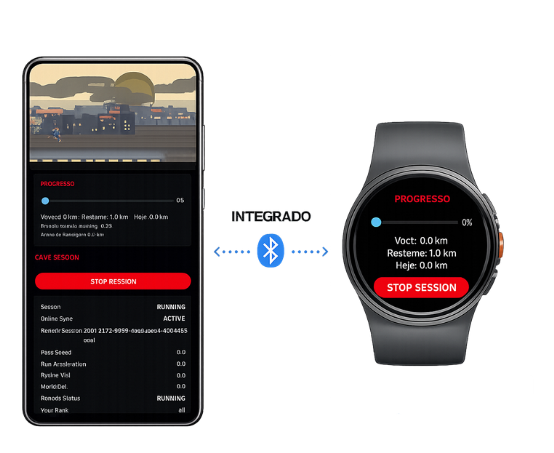
\includegraphics[width=0.9\textwidth]{figuras/aplicativo_relogio.png}
    \captionsetup{justification=centering}
    \caption{Interface do aplicativo móvel conectado ao relógio via Bluetooth.}
    \label{fig:aplicativo-relogio}
\end{figure*}

Posteriormente, a estratégia de coleta de localização foi modificada. Como o relógio utilizado nos testes foi um \textit{Samsung Galaxy Watch 6} pareado ao celular, era necessário manter o \textit{smartphone} próximo ao \textit{smartwatch} durante a execução da atividade. Dessa forma, optou-se por centralizar a coleta de GPS no aplicativo móvel, solução que apresentou maior viabilidade para os testes em campo e melhor precisão no contexto da arquitetura proposta.

A Figura~\ref{fig:grafico_frequencia} apresenta a frequência cardíaca coletada pelo \textit{smartwatch} durante a sessão de corrida. Esse dado representa a principal informação biométrica utilizada no sistema e contribui para o acompanhamento da atividade durante a execução.

Também foram observados desafios na comunicação entre os dispositivos e o \textit{backend}. Em alguns testes, as respostas recebidas do servidor nem sempre refletiam de maneira coerente o estado observado durante a execução. Esse comportamento evidenciou a importância de tratar o \textit{backend} como fonte autoritativa da sessão e de manter o aplicativo móvel responsável pela renderização do estado recebido, reduzindo interpretações locais divergentes dos dados.

De forma geral, a análise funcional indica que os três componentes principais operam de maneira integrada. O relógio fornece dados biométricos, o aplicativo móvel centraliza a experiência do usuário e o \textit{backend} coordena o estado autoritativo da corrida. Essa divisão reforça a plausibilidade da arquitetura proposta para sustentar uma experiência gamificada em tempo real, ainda que melhorias futuras sejam necessárias para ampliar a robustez das validações em campo, a sincronização entre dispositivos e a comprovação com diferentes modelos de \textit{smartwatch}.